\section{Results and Analysis}

\begin{table*}[t]
\centering
\small
\begin{tabular}{lrrrr}
\toprule
Model & Parse & Function & Arguments & Exact Call \\
\midrule
BabyA JSON & 0.0187 & 0.0031 & 0.0000 & 0.0000 \\
BabyB JSON & 0.3559 & 0.0531 & 0.0000 & 0.0000 \\
FunctionGemma 270M & 0.9813 & 0.7097 & 0.5099 & 0.4964 \\
BabyA DSL & 0.3632 & 0.0000 & 0.0937 & 0.0000 \\
BabyB DSL & 0.1145 & 0.0083 & 0.0250 & 0.0073 \\
\bottomrule
\end{tabular}
\caption{Official Mobile Actions evaluation results on 961 examples. Exact call requires both function name and full argument dictionary to match.}
\label{tab:main-results}
\end{table*}

Table~\ref{tab:main-results} gives the main result. BabyB is much better than BabyA under the same JSON setup, especially on parse rate and function accuracy. This supports the central pretraining hypothesis in a limited comparative sense: the stronger Baby model moves closer to structured parsing. However, the task remains unsolved for both Baby models. BabyB often produces parseable JSON fragments, but it does not produce exact full tool calls.

\begin{figure}[t]
\centering
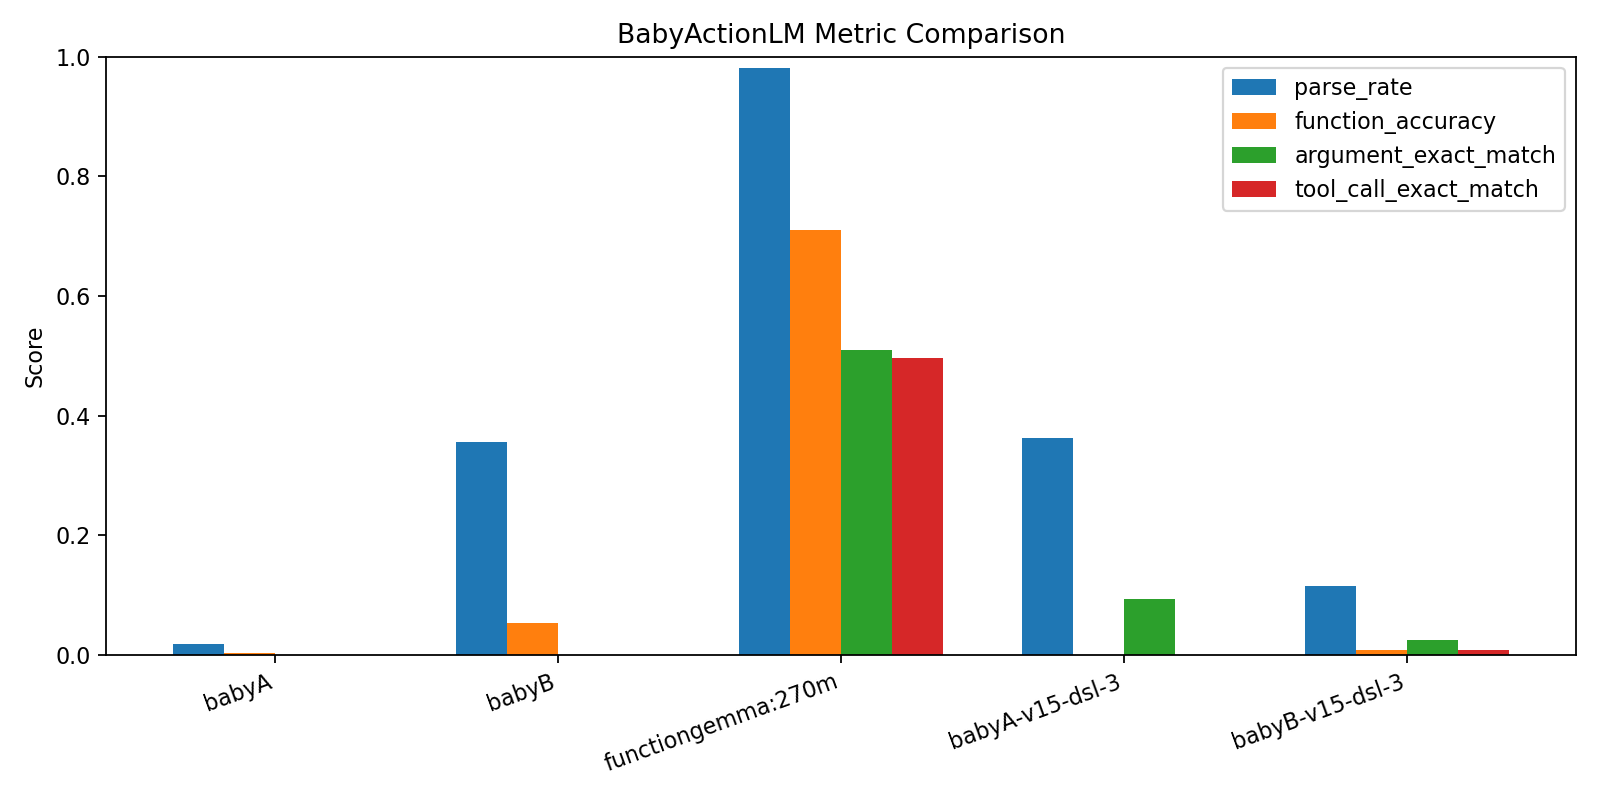
\includegraphics[width=\columnwidth]{figures/metric_comparison.png}
\caption{Metric comparison across BabyA, BabyB, the DSL diagnostic runs, and FunctionGemma.}
\label{fig:metrics}
\end{figure}

Figure~\ref{fig:metrics} highlights the gap between the fine-tuned Baby checkpoints and FunctionGemma. FunctionGemma reaches 98.1\% parse rate and 49.6\% exact tool-call match. This shows that the dataset and metric are meaningful: the task is not impossible, but it is far beyond what the current BabyA/B fine-tuning setup can reliably solve.

\begin{figure}[t]
\centering
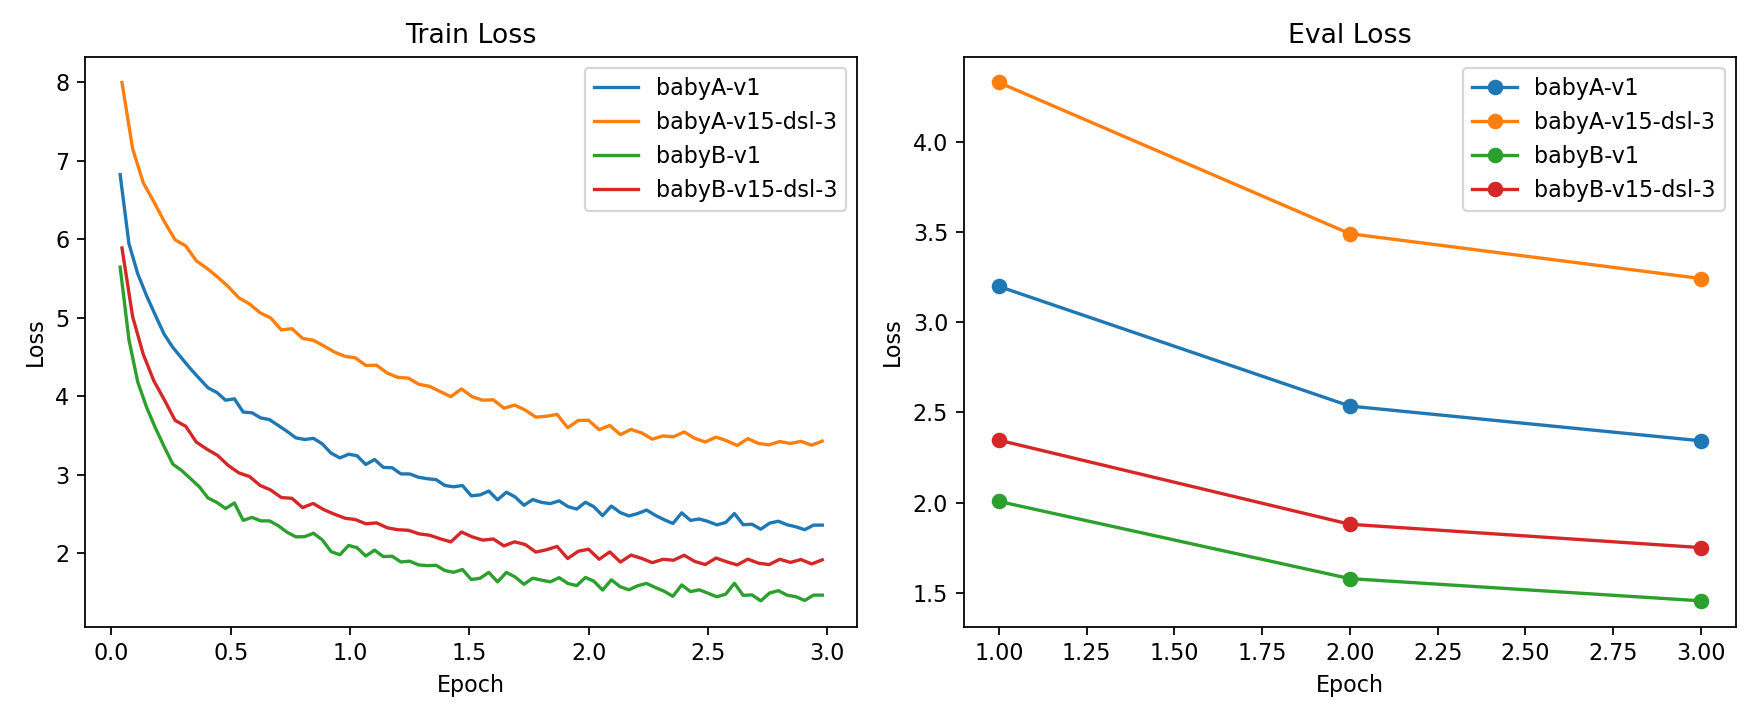
\includegraphics[width=\columnwidth]{figures/training_curves.png}
\caption{Fine-tuning loss curves for JSON and selected DSL BabyA/B runs. BabyB reaches lower evaluation loss than BabyA, but lower loss does not imply reliable exact tool calls.}
\label{fig:training}
\end{figure}

The training curves in Figure~\ref{fig:training} provide another view of the BabyA/B difference. BabyB reaches lower evaluation loss than BabyA in both target formats. This is consistent with the metric advantage in Table~\ref{tab:main-results}, but also shows the limit of token-level training loss as a proxy for structured correctness: exact arguments remain fragile even when loss decreases.

\paragraph{Format sensitivity.}
The format-selection trial gives partial support to the output-format hypothesis. On the BabyB development split, the 3-epoch DSL setup is the only variant with nonzero exact match, 0.0080, while the longer JSON run has better parse and function scores but still 0 exact match. On official eval, BabyB with the selected DSL target reaches 0.0073 exact match. This is a real but tiny signal. The honest interpretation is that target format matters, but a flatter string format does not solve mobile tool-call parsing for these models. BabyA with the same DSL target is especially cautionary: it reaches 36.3\% parse rate but 0 function accuracy, so parseability alone is not semantic success.

\paragraph{Per-tool behavior.}
The per-tool results show that BabyB's JSON function accuracy is concentrated in \texttt{show\_map}: 34.5\% function accuracy for that tool, while the other tools are effectively 0. FunctionGemma is strong across simple tools, especially flashlight and Wi-Fi actions, but argument-heavy tools such as contact creation and email remain harder. This suggests that copying or normalizing arguments is a separate challenge from choosing the action type.

\begin{table}[t]
\centering
\small
\begin{tabular}{p{0.28\columnwidth}p{0.62\columnwidth}}
\toprule
Field & Text \\
\midrule
Command & Show the location of the Rijksmuseum in Amsterdam on the map. \\
Gold & Tool: \texttt{show\_map}; query: Rijksmuseum in Amsterdam. \\
BabyB JSON & Tool: \texttt{show\_map}; query: \texttt{mail-020-101-10t10:00:00}. \\
\bottomrule
\end{tabular}
\caption{Qualitative BabyB example. The tool name is correct, but the argument is unrelated to the command.}
\label{tab:qual}
\end{table}

Table~\ref{tab:qual} shows the common partial-learning pattern. BabyB identifies that a location request should call \texttt{show\_map}, but it fails to copy the requested location into the argument. This explains why function accuracy can improve while argument exact match remains 0.
